\section{Layanan Pendukung}

Setiap arsitektur solusi berkomunikasi dengan dua layanan lain, yaitu layanan pengguna dan layanan pembayaran. Solusi yang berkomunikasi dengan layanan ini akan diusahakan sehingga tidak menjadi sumber \textit{bottleneck}. Berikut adalah detail dari kedua layanan tersebut:

\subsection{Layanan Pengguna}

Layanan ini merupakan \textit{instance} Ory Kratos, sebuah solusi yang menawarkan manajemen pengguna \textit{out of the box} seperti Keycloak. Layanan pengguna tidak akan menjadi \textit{bottleneck} karena pada saat pengujian, akan diasumsikan seluruh pengguna sudah \textit{login} dan pemeriksaan otentikasi dilakukan pada masing-masing \textit{instance backend}. Layanan ini terhubung dengan sebuah basis data untuk menyimpan data pengguna. Basis data yang akan digunakan adalah PostgreSQL. \textit{Instance} basis data ini akan dibuat terpisah dengan basis data yang digunakan oleh sistem tiket. Penskalaan pada arsitektur ini cukup dengan menambah jumlah \textit{instance} yang berjalan (penskalaan secara horizontal).

\begin{figure}[htbp]
    \centering
    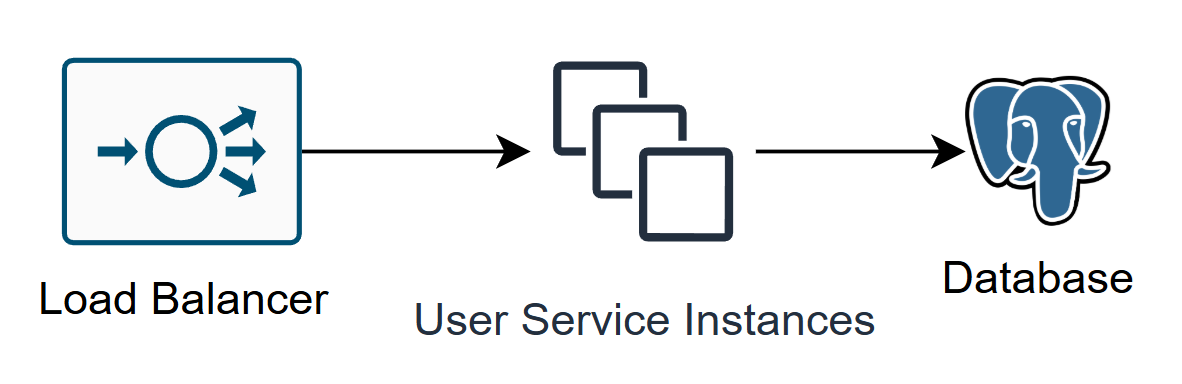
\includegraphics[width=0.8\textwidth]{resources/appendix/user-service.png}
    \caption{Arsitektur Layanan Pengguna}
    \label{fig:user-service-deployment}
\end{figure}

\subsection{Layanan Pembayaran}

Layanan ini merupakan \textit{mock service} gerbang pembayaran. Layanan ini berpotensi menjadi sumber \textit{bottleneck} saat proses pembuatan tagihan, terlebih lagi karena komunikasi pembuatan tagihan harus dilakukan secara sinkron. Untuk memastikan \textit{throughput} yang tinggi, layanan ini akan menggunakan \textit{in-memory database} dengan \textit{persistence} seperti Redis. Redis akan dikonfigurasikan dalam mode kluster untuk kebutuhan \textit{sharding} dan \textit{multiple writer}. \textit{Persistence} dan \textit{snapshot} masih akan dikonfigurasikan, meski tetap akan ada periode waktu yang bisa mengakibatkan terjadinya \textit{data loss} (kurang dari satu detik). Skenario pengujian akan mengasumsikan tidak terjadinya kegagalan pada layanan ini, sehingga tidak ada data yang hilang.

Ketika pembayaran berhasil atau kadaluarsa, layanan ini akan memanggil \textit{webhook} pada layanan tiket. Untuk memastikan pemberitahuan terkirim, layanan ini akan melakukan \textit{retry} ketika terjadi kegagalan saat pemanggilan \textit{webhook}. Komponen \textit{timer} untuk \textit{expiration} dan \textit{queue} untuk pemanggilan \textit{webhook} juga akan menggunakan Redis.

Komponen pada layanan ini akan dibagi menjadi dua, yaitu \textit{payment processor} dan \textit{notifier}. \textit{Payment processor} merupakan komponen yang melayani pembuatan tagihan dan pembayaran tagihan. \textit{Notifier} merupakan komponen yang menangani \textit{timer} ketika terdapat pembayaran yang kadaluarsa dan  memanggil \textit{webhook} ketika pembayaran berhasil atau kadaluarsa. Setiap komponen dapat di-\textit{scale} secara horizontal.

\begin{figure}[htbp]
    \centering
    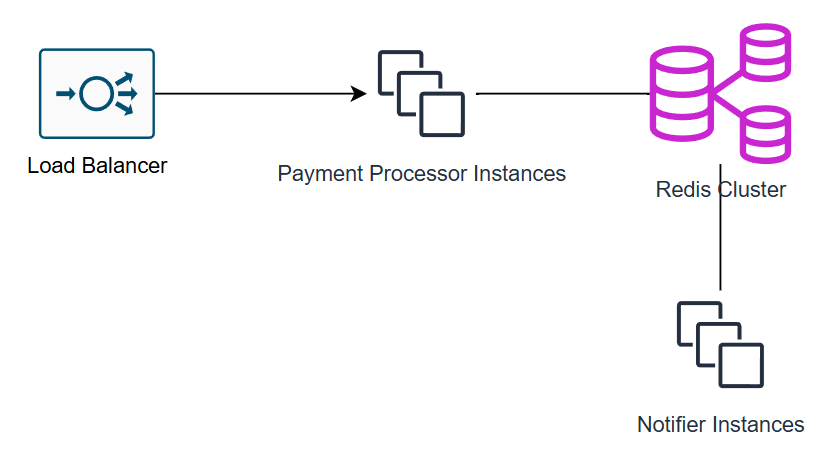
\includegraphics[width=0.8\textwidth]{resources/appendix/payment-service.png}
    \caption{Arsitektur Layanan Pembayaran}
    \label{fig:payment-service-deployment}
\end{figure}
